% DISCOVERY CURRICULUM — Journey 1, Module 3
% "Graphs as Structures"
% Compile: pdflatex J1_M3.tex (twice)

\documentclass[12pt, a4paper]{article}

\usepackage[a4paper, top=2.8cm, bottom=2.8cm, left=3.0cm, right=2.5cm, includeheadfoot, headheight=15pt]{geometry}
\usepackage{amsmath, amsthm}
\usepackage[charter, cal=cmcal]{mathdesign}
\usepackage[scaled=0.92]{helvet}
\usepackage{xcolor}
\usepackage{tcolorbox}
\tcbuselibrary{skins, breakable, theorems}
\usepackage{enumitem}
\usepackage{graphicx}
\usepackage{tikz}
\usetikzlibrary{arrows.meta, positioning, calc}
\usepackage{pgfplots}
\pgfplotsset{compat=1.18}
\usepackage{booktabs}
\usepackage{array}
\usepackage{fancyhdr}
\usepackage{titlesec}
\usepackage{parskip}
\usepackage{microtype}
\usepackage{hyperref}
\hypersetup{colorlinks=true, linkcolor=NavyBlue, urlcolor=NavyBlue}

% ── Colours ─────────────────────────────────────────────────
\definecolor{NavyBlue}{HTML}{1E3A8A}
\definecolor{MidBlue}{HTML}{2E6DA4}
\definecolor{Gold}{HTML}{D97706}
\definecolor{LightBlue}{HTML}{EFF6FF}
\definecolor{LightGold}{HTML}{FEF3C7}
\definecolor{DarkGrey}{HTML}{334155}
\definecolor{BoxGreen}{HTML}{F0FDF4}
\definecolor{SoftRed}{HTML}{FFF1F2}
\definecolor{SidebarGrey}{HTML}{F8FAFC}

% ── Section formatting ───────────────────────────────────────
\titleformat{\section}{\Large\bfseries\color{NavyBlue}}{}{0em}{}[{\color{MidBlue}\vspace{2pt}\rule{\linewidth}{1.5pt}}]
\titleformat{\subsection}{\large\bfseries\color{MidBlue}}{}{0em}{}
\titleformat{\subsubsection}{\normalsize\bfseries\color{Gold}}{}{0em}{}

% ── Header / Footer ─────────────────────────────────────────
\pagestyle{fancy}
\fancyhf{}
\fancyhead[L]{\small\color{DarkGrey}\textit{Discovery Curriculum}}
\fancyhead[R]{\small\color{DarkGrey}\textit{Journey 1 $\cdot$ Module 3}}
\fancyfoot[C]{\small\color{MidBlue}\thepage}
\renewcommand{\headrulewidth}{0.4pt}

% ── Environments (tcolorbox Unification) ─────────────────────

% Puzzle box — opening problem
\newtcolorbox{puzzlebox}[1][]{
  enhanced, breakable,
  colback=NavyBlue!5, colframe=NavyBlue,
  boxrule=0pt, leftrule=2.5pt,
  sharp corners,
  left=12pt, right=10pt, top=10pt, bottom=10pt,
  before skip=14pt, after skip=10pt,
  #1
}

% Discovery box — moment of crystallisation
\newtcolorbox{discoverybox}[1][]{
  enhanced, breakable,
  colback=LightGold, colframe=Gold,
  boxrule=0pt, leftrule=2.5pt,
  sharp corners,
  left=12pt, right=10pt, top=10pt, bottom=10pt,
  before skip=14pt, after skip=10pt,
  #1
}

% Name box — formal definition reveal
\newtcolorbox{namebox}[1][]{
  enhanced, breakable,
  colback=LightBlue, colframe=MidBlue,
  boxrule=0.8pt,
  arc=4pt,
  left=12pt, right=10pt, top=10pt, bottom=10pt,
  before skip=14pt, after skip=10pt,
  #1
}

% Reflection box
\newtcolorbox{reflectionbox}[1][]{
  enhanced, breakable,
  colback=BoxGreen, colframe=DarkGrey!35,
  boxrule=0.8pt,
  arc=4pt,
  left=12pt, right=10pt, top=10pt, bottom=10pt,
  before skip=14pt, after skip=10pt,
  #1
}

% Thought provocation — inline philosophical aside
\newtcolorbox{thought}[1][]{
  enhanced, breakable,
  colback=SidebarGrey, colframe=Gold,
  boxrule=0pt, leftrule=1.5pt,
  sharp corners,
  left=10pt, right=10pt, top=7pt, bottom=7pt,
  before skip=10pt, after skip=10pt,
  #1
}

% Problem counter
\newcounter{problem}
\newenvironment{problem}[1][]{%
  \refstepcounter{problem}%
  \par\vspace{6pt}%
  \noindent\textbf{\color{MidBlue}Problem \theproblem}%
  \ifx&#1&\else\ \textit{(#1)}\fi\textbf{.}\enskip
}{\par\vspace{4pt}}

% Deep problem counter
\newcounter{deepproblem}
\newenvironment{deepproblem}[1][]{%
  \refstepcounter{deepproblem}%
  \par\vspace{6pt}%
  \noindent\textbf{\color{NavyBlue}$\bigstar$\ Deep Problem \thedeepproblem}%
  \ifx&#1&\else\ \textit{(#1)}\fi\textbf{.}\enskip
}{\par\vspace{4pt}}

% Exercise counter
\newcounter{exercise}
\newenvironment{exercise}[1][]{%
  \refstepcounter{exercise}%
  \par\vspace{6pt}%
  \noindent\textbf{\color{Gold}Exercise \theexercise}%
  \ifx&#1&\else\ \textit{(#1)}\fi\textbf{.}\enskip
}{\par\vspace{4pt}}

\tikzset{
  vx/.style={circle,draw=NavyBlue,fill=LightBlue,thick,minimum size=7mm,
             font=\small\bfseries,text=NavyBlue},
  ed/.style={MidBlue,thick},
  ded/.style={MidBlue,thick,-{Stealth[length=5pt]}}
}

\begin{document}

% Cover
\thispagestyle{empty}
\begin{center}
{\small\color{MidBlue}\textbf{DISCOVERY CURRICULUM}\quad$\cdot$\quad\textbf{JOURNEY 1: REPRESENTATION}}
\vspace{0.6cm}

{\color{NavyBlue}\rule{\linewidth}{2pt}}
\vspace{0.5cm}

{\Huge\bfseries\color{NavyBlue}Module 3}\\[0.3cm]
{\LARGE\bfseries\color{MidBlue}Graphs as Structures}\\[0.4cm]
{\color{Gold}\rule{0.4\linewidth}{1.2pt}}\\[0.4cm]
{\large\itshape\color{DarkGrey}Not every relationship can be captured by a formula.\\[0.15cm]
Some things are about \emph{connection}, not quantity.}

\vspace{1cm}
\begin{tabular}{rl}
\color{DarkGrey}\textbf{Journey}           & Journey 1 --- Representation \\[4pt]
\color{DarkGrey}\textbf{Module}            & 3 of 6 \\[4pt]
\color{DarkGrey}\textbf{Prerequisites}     & Modules 1--2 \\[4pt]
\color{DarkGrey}\textbf{You will discover} & Graphs, degree, paths, trees, adjacency matrices \\[4pt]
\color{DarkGrey}\textbf{Format}            & 8 problems $+$ 3 deep problems $\approx$ 13--15 pages \\
\end{tabular}
\vspace{1cm}

{\color{NavyBlue}\rule{\linewidth}{2pt}}
\end{center}

\vspace{0.5cm}
\noindent\textbf{Recap of Modules 1--2.}
So far you have been building a language for \emph{functional} relationships: rules that assign exactly one output to each input. But many important relationships in the world are not functional. A friendship is not a function. A road network is not a function. The bonds holding a molecule together are not a function. These relationships are about \emph{connection} between objects, not about computing outputs.

\medskip
This module introduces the \textbf{graph}: a representational tool built precisely for these structures. The graph will turn out to connect to functions and linear algebra in a surprising way --- through the adjacency matrix, which translates connection into multiplication.

\newpage

\section{Part 1 --- The Puzzle}

\begin{puzzlebox}
\textbf{The Opening Puzzle: K\"{o}nigsberg.}

The city of K\"{o}nigsberg (now Kaliningrad, Russia) sits on two islands in the Pregel river. In the 18th century, seven bridges connected the islands to each other and to the two riverbanks.

\begin{center}
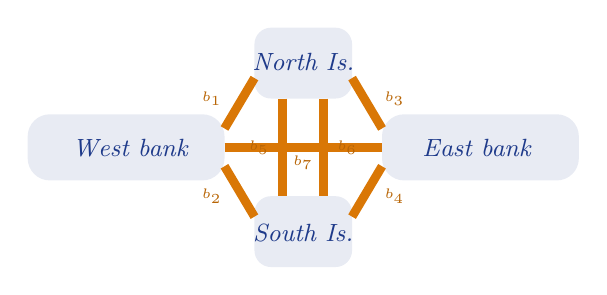
\begin{tikzpicture}[scale=1.0]
  \fill[NavyBlue!10, rounded corners=8pt] (-3.5,-0.42) rectangle (-1.0, 0.42);
  \fill[NavyBlue!10, rounded corners=8pt] ( 1.0,-0.42) rectangle ( 3.5, 0.42);
  \fill[NavyBlue!10, rounded corners=6pt] (-0.62,-1.52) rectangle (0.62,-0.62);
  \fill[NavyBlue!10, rounded corners=6pt] (-0.62, 0.62) rectangle (0.62, 1.52);

  \node[font=\small\itshape,color=NavyBlue] at (-2.2,0)   {West bank};
  \node[font=\small\itshape,color=NavyBlue] at ( 2.2,0)   {East bank};
  \node[font=\small\itshape,color=NavyBlue] at (0,-1.08)  {South Is.};
  \node[font=\small\itshape,color=NavyBlue] at (0, 1.08)  {North Is.};

  \draw[Gold,line width=3.2pt] (-1.0, 0.24) -- (-0.62, 0.88);
  \draw[Gold,line width=3.2pt] (-1.0,-0.24) -- (-0.62,-0.88);
  \draw[Gold,line width=3.2pt] ( 1.0, 0.24) -- ( 0.62, 0.88);
  \draw[Gold,line width=3.2pt] ( 1.0,-0.24) -- ( 0.62,-0.88);
  \draw[Gold,line width=3.2pt] (-0.26, 0.62) -- (-0.26,-0.62);
  \draw[Gold,line width=3.2pt] ( 0.26, 0.62) -- ( 0.26,-0.62);
  \draw[Gold,line width=3.2pt] (-1.0, 0) -- ( 1.0, 0);

  \node[font=\tiny,color=Gold!85!black] at (-1.16, 0.62)  {$b_1$};
  \node[font=\tiny,color=Gold!85!black] at (-1.16,-0.62)  {$b_2$};
  \node[font=\tiny,color=Gold!85!black] at ( 1.16, 0.62)  {$b_3$};
  \node[font=\tiny,color=Gold!85!black] at ( 1.16,-0.62)  {$b_4$};
  \node[font=\tiny,color=Gold!85!black] at (-0.56, 0.0)   {$b_5$};
  \node[font=\tiny,color=Gold!85!black] at ( 0.56, 0.0)   {$b_6$};
  \node[font=\tiny,color=Gold!85!black] at ( 0.0, -0.20)  {$b_7$};
\end{tikzpicture}
\end{center}

\textbf{Question.} Is it possible to walk through the city crossing each bridge exactly once? You may start and end anywhere. Try it. Can you prove your answer?
\end{puzzlebox}

\medskip
This puzzle was posed to \textbf{Leonhard Euler} in 1736. His solution is the founding moment of graph theory and topology. The key was not to search harder for a route --- it was to \emph{change the representation}: discard all geometry, keep only what is connected to what.

\begin{thought}
\textbf{The power of the right representation.}
Many hard problems become easy once you represent them correctly. The K\"{o}nigsberg problem looks like a geography puzzle. It is not. It is a question about the combinatorial structure of connections. Strip away the riverbanks, the bridge lengths, the shape of the city --- what remains is a tiny diagram of dots and lines, and in that diagram the answer becomes almost immediate. This is one of the deepest lessons in mathematics: before you solve a problem, ask whether you are looking at it in the right language.
\end{thought}

\section{Part 2 --- Exploration}

\subsection{Step 1: Stripping away geometry}

\begin{problem}
\label{prob:konigsberg}
Replace each land mass with a point (a \emph{vertex}) and each bridge with a line segment (an \emph{edge}) joining the two land masses it connects.
\begin{enumerate}[label=(\alph*),topsep=2pt]
  \item Draw the diagram. You should have 4 vertices and 7 edges.
  \item Count the number of edges at each vertex. (This is the \emph{degree} of that vertex.)
  \item List the four degrees. What do you notice?
  \item A walk using every edge exactly once is called an \emph{Eulerian path}. Based on the degrees, form a hypothesis: what property might determine whether one exists?
\end{enumerate}
\end{problem}

\begin{center}
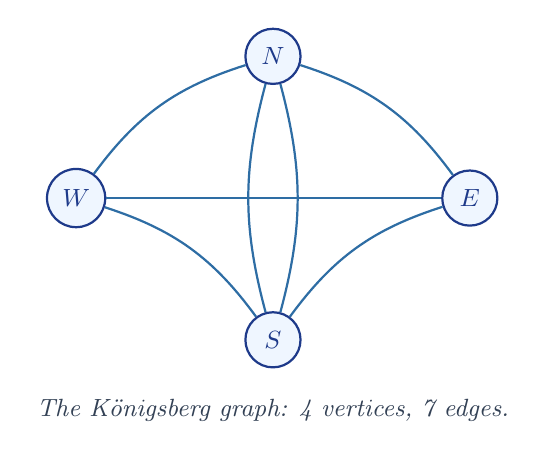
\begin{tikzpicture}
  \node[vx] (W) at (-2.5,  0)  {$W$};
  \node[vx] (E) at ( 2.5,  0)  {$E$};
  \node[vx] (N) at ( 0,  1.8)  {$N$};
  \node[vx] (S) at ( 0, -1.8)  {$S$};

  \draw[ed] (W) to[bend left=18]  (N);
  \draw[ed] (W) to[bend left=18]  (S);
  \draw[ed] (E) to[bend right=18] (N);
  \draw[ed] (E) to[bend right=18] (S);
  \draw[ed] (N) to[bend left=15]  (S);
  \draw[ed] (N) to[bend right=15] (S);
  \draw[ed] (W) -- (E);

  \node[font=\small\itshape,color=DarkGrey] at (0,-2.7)
    {The K\"{o}nigsberg graph: 4 vertices, 7 edges.};
\end{tikzpicture}
\end{center}

\begin{thought}
\textbf{What abstraction keeps and what it discards.}
The graph above has thrown away every piece of geographical information: the shape of the islands, the width of the river, the length of each bridge. None of that is needed. What the graph preserves is the only thing that matters: which land masses are connected, and how many times. The question to always ask is not ``what can I add to make this richer?'' but ``what can I safely remove without losing the answer?''
\end{thought}

\begin{problem}
\label{prob:examples}
For each situation, draw a graph. Decide what vertices and edges represent, and whether edges need directions.
\begin{enumerate}[label=(\alph*),topsep=2pt]
  \item Five people. Edges mean ``has shaken hands with.''
  \item Four cities. Edges mean ``there is a direct bus route.''
  \item A set of web pages. Edges mean ``this page links to that one.''
  \item Tasks in a project. Edges mean ``must be completed before.''
  \item The integers $\{1,2,3,4,5,6\}$. Connect $a$ to $b$ if $a$ divides $b$.
\end{enumerate}
For each: can an edge go from a vertex to itself? Can two vertices share more than one edge?
\end{problem}

\subsection{Step 2: Measuring graphs}

\begin{problem}
\label{prob:degree}
Let $G$ have vertices $\{A,B,C,D,E\}$ and edges $\{AB, BC, CD, DE, EA, AC, BD\}$.

\begin{center}
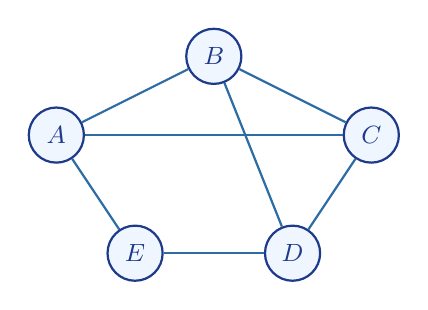
\begin{tikzpicture}
  \node[vx] (A) at (0,  0)   {$A$};
  \node[vx] (B) at (2,  1)   {$B$};
  \node[vx] (C) at (4,  0)   {$C$};
  \node[vx] (D) at (3,-1.5)  {$D$};
  \node[vx] (E) at (1,-1.5)  {$E$};
  \draw[ed] (A)--(B); \draw[ed] (B)--(C); \draw[ed] (C)--(D);
  \draw[ed] (D)--(E); \draw[ed] (E)--(A); \draw[ed] (A)--(C);
  \draw[ed] (B)--(D);
\end{tikzpicture}
\end{center}

\begin{enumerate}[label=(\alph*),topsep=2pt]
  \item Write the degree of each vertex.
  \item Sum all degrees. How does this relate to the number of edges?
  \item \textit{Prove} that in any graph, the sum of all degrees equals $2|E|$. \textit{Hint: what does each edge contribute to the degree count?}
  \item Deduce that in any graph, the number of odd-degree vertices is even.
  \item How does (d) immediately resolve the K\"{o}nigsberg puzzle?
\end{enumerate}
\end{problem}

The result in (c) is the \textbf{handshaking lemma}. If vertices are people and edges are handshakes: the total count of ``hands shaken'' (summing everyone's count) equals twice the number of handshakes. Clean, inevitable, and powerful.

\subsection{Step 3: Moving through graphs}

\begin{problem}
\label{prob:paths}
A \textbf{path} is a sequence $v_0, v_1, \ldots, v_k$ with each consecutive pair connected by an edge. A \textbf{cycle} is a path returning to its start.
\begin{enumerate}[label=(\alph*),topsep=2pt]
  \item In the graph from Problem~\ref{prob:degree}: find a path from $A$ to $D$. Is it unique?
  \item Find a cycle visiting every vertex exactly once (a \emph{Hamiltonian cycle}), or prove none exists.
  \item A graph is \textbf{connected} if every pair of vertices is linked by some path. Is this graph connected?
  \item Draw a disconnected graph. How many edges must you add to make it connected?
  \item A \textbf{tree} is a connected graph with no cycles. Draw three trees on 5 vertices. How many edges does each have? Conjecture a general rule.
\end{enumerate}
\end{problem}

\begin{center}
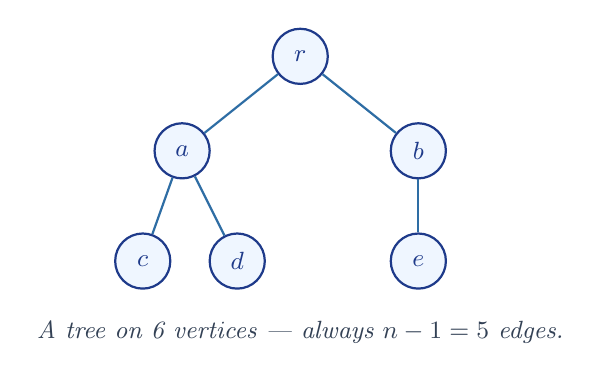
\begin{tikzpicture}
  \node[vx] (r) at (2,  2)   {$r$};
  \node[vx] (a) at (0.5,0.8) {$a$};
  \node[vx] (b) at (3.5,0.8) {$b$};
  \node[vx] (c) at (0, -0.6) {$c$};
  \node[vx] (d) at (1.2,-0.6){$d$};
  \node[vx] (e) at (3.5,-0.6){$e$};
  \draw[ed] (r)--(a); \draw[ed] (r)--(b);
  \draw[ed] (a)--(c); \draw[ed] (a)--(d); \draw[ed] (b)--(e);
  \node[font=\small\itshape,color=DarkGrey] at (2,-1.5)
    {A tree on 6 vertices --- always $n-1 = 5$ edges.};
\end{tikzpicture}
\end{center}

\begin{thought}
\textbf{Trees are everywhere.}
Trees arise wherever structure is hierarchical: family genealogies, file systems, parse trees in linguistics, decision trees in machine learning, evolutionary trees in biology, the branching of blood vessels and river deltas. The mathematical property making them special --- a tree on $n$ vertices always has exactly $n-1$ edges --- is fundamental in algorithm design. The shortest-path algorithms that power GPS navigation and internet routing are built on spanning trees. The probability trees you will meet in Journey~5 are the same combinatorial object in a different context.
\end{thought}

\subsection{Step 4: Graphs as matrices}

This is where graph structure and linear algebra first meet.

\begin{problem}
\label{prob:adjacency}
For a graph with $n$ vertices labelled $1, \ldots, n$, define the \textbf{adjacency matrix} $A$ by
\[
  A_{ij} = \begin{cases} 1 & \text{if vertices } i \text{ and } j \text{ share an edge,} \\ 0 & \text{otherwise.} \end{cases}
\]
\begin{enumerate}[label=(\alph*),topsep=2pt]
  \item Write the adjacency matrix of the graph from Problem~\ref{prob:degree} (label $A=1, B=2, C=3, D=4, E=5$).
  \item What symmetry does $A$ have? Why must this hold for any undirected graph?
  \item Compute $A^2$. Verify the entry $(A^2)_{13}$ by manually counting all walks of length 2 from vertex 1 to vertex 3. What does $(A^2)_{ij}$ count in general?
  \item What does $(A^k)_{ij}$ count? State a general conjecture.
  \item What is the sum of row $i$? Which graph property does this recover?
\end{enumerate}
\end{problem}

\begin{thought}
\textbf{Structure encoded as numbers.}
The adjacency matrix takes a combinatorial structure --- dots and lines --- and converts it into an array of numbers amenable to multiplication and decomposition. Once you have the matrix, all of linear algebra becomes available. The eigenvalues of $A$ (Journey~3) reveal deep properties: how fast information spreads, how strongly communities cluster, how quickly a random walk mixes. Google's PageRank algorithm ranks web pages by computing eigenvectors of a matrix encoding the entire hyperlink structure of the web. A billion-dollar idea, rooted exactly here.
\end{thought}

\begin{problem}
\label{prob:directed}
A \textbf{directed graph} (digraph) has directed edges; $u \to v$ differs from $v \to u$.

\begin{center}
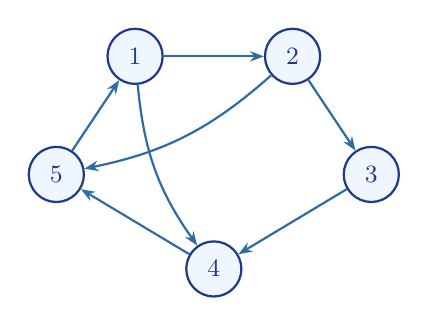
\begin{tikzpicture}
  \node[vx] (1) at (0,  1.5) {$1$};
  \node[vx] (2) at (2,  1.5) {$2$};
  \node[vx] (3) at (3,  0)   {$3$};
  \node[vx] (4) at (1, -1.2) {$4$};
  \node[vx] (5) at (-1, 0)   {$5$};
  \draw[ded] (1)--(2); \draw[ded] (2)--(3); \draw[ded] (3)--(4);
  \draw[ded] (4)--(5); \draw[ded] (5)--(1);
  \draw[ded] (1) to[bend right=15] (4);
  \draw[ded] (2) to[bend left=15]  (5);
\end{tikzpicture}
\end{center}

\begin{enumerate}[label=(\alph*),topsep=2pt]
  \item Write the adjacency matrix. Is it symmetric?
  \item Define \textbf{in-degree} (edges arriving) and \textbf{out-degree} (edges leaving). Compute both for each vertex.
  \item Is there a directed path from vertex~1 to vertex~3? From 3 to 1?
  \item A digraph is \textbf{strongly connected} if directed paths exist between every ordered pair of vertices. Is this one strongly connected?
  \item Can you interpret a directed graph as a function from some set to some other set? What would domain and codomain be?
\end{enumerate}
\end{problem}

\begin{problem}
\label{prob:counting}
\begin{enumerate}[label=(\alph*),topsep=2pt]
  \item What is the maximum number of edges in a graph on $n$ vertices (no self-loops, no repeated edges)?
  \item The \textbf{complete graph} $K_n$ connects every pair. Draw $K_3, K_4, K_5$. How many edges does $K_n$ have?
  \item A graph is \textbf{bipartite} if its vertices split into two groups so every edge goes between groups. Give two real-life examples.
  \item Draw $K_{3,3}$: 3 left vertices, 3 right, every left connected to every right. Can you draw it without edge crossings?
  \item Can you draw $K_5$ in the plane without crossings?
\end{enumerate}
\end{problem}

\begin{thought}
\textbf{Planarity and circuit design.}
Whether a graph can be drawn without edge crossings is called \textbf{planarity}. In printed circuit board design, crossing conducting traces can short-circuit. A circuit laid out flat without crossings corresponds to a planar graph. Kuratowski's theorem (1930) proves $K_{3,3}$ and $K_5$ are not planar. This is why complex circuits require multiple stacked layers --- the crossing constraint cannot be avoided on a single plane. Modern processors contain tens of billions of transistors spread across dozens of metal layers, each layer a planar graph. Every layer is an engineering response to the non-planarity problem you just encountered in (d) and (e).
\end{thought}

\section{Part 3 --- Discovery}

\begin{discoverybox}
\textbf{What have we built?}

\begin{enumerate}
  \item A \textbf{graph} captures pure connection, stripped of all geometry.
  \item The \textbf{handshaking lemma} (sum of degrees $= 2|E|$) constrains all possible walks. Euler's theorem follows: an Eulerian path exists if and only if there are 0 or 2 odd-degree vertices.
  \item \textbf{Trees} are minimally connected graphs. A tree on $n$ vertices has exactly $n-1$ edges.
  \item The \textbf{adjacency matrix} translates graph structure into linear algebra. Powers count paths.
\end{enumerate}

\textbf{Before reading on.} Using the handshaking lemma and the degrees from Problem~\ref{prob:konigsberg}: write a complete, careful proof that no Eulerian path exists in K\"{o}nigsberg.
\end{discoverybox}

\section{Part 4 --- Naming the Ideas}

\begin{namebox}
\textbf{Graphs: formal definition.}

A \textbf{graph} $G = (V, E)$ has a vertex set $V$ and edge set $E$, where each edge is an unordered pair $\{u,v\}$ of distinct vertices. The \textbf{degree} $\deg(v)$ is the number of edges containing $v$.

\medskip
\textbf{Handshaking Lemma.} $\displaystyle\sum_{v \in V} \deg(v) = 2|E|$.

\medskip
\textbf{Euler's Theorem (1736).} A connected graph has an Eulerian path if and only if it has exactly 0 or 2 vertices of odd degree. It has an Eulerian \emph{circuit} (returning to start) if and only if \emph{every} vertex has even degree.
\end{namebox}

\begin{namebox}
\textbf{Trees.}

A \textbf{tree} is a connected acyclic graph. The following are equivalent for a graph on $n$ vertices:
\begin{itemize}[topsep=3pt]
  \item $G$ is a tree.
  \item $G$ is connected with $n-1$ edges.
  \item $G$ is acyclic with $n-1$ edges.
  \item There is a unique path between any two vertices.
\end{itemize}
Every connected graph contains a \textbf{spanning tree}: a subgraph that is a tree on all $n$ vertices.
\end{namebox}

\begin{namebox}
\textbf{The adjacency matrix and spectral graph theory.}

The \textbf{adjacency matrix} $A$ has $A_{ij} = 1$ if $\{i,j\} \in E$, else $0$. The entry $(A^k)_{ij}$ counts walks of length $k$ from $i$ to $j$.

The \textbf{eigenvalues} of $A$ (to be developed in Journey~3) encode structural properties:
\begin{itemize}[topsep=3pt]
  \item The largest eigenvalue $\lambda_1$ relates to overall connectivity.
  \item The second eigenvalue $\lambda_2$ controls random-walk mixing (central in Journey~5).
  \item The full eigenvalue list is the graph's \textbf{spectrum}.
\end{itemize}
This field is \textbf{spectral graph theory}. It underlies PageRank, community detection, and social-network analysis.
\end{namebox}

\section{Part 5 --- Deep Problems}

\begin{deepproblem}[Euler's theorem, complete proof]
\begin{enumerate}[label=(\alph*)]
  \item Prove the necessary direction: if an Eulerian path exists, at most 2 vertices have odd degree. \textit{Hint: consider what happens to degree parity as the path enters and leaves each vertex.}
  \item Prove the sufficient direction: if the graph is connected with 0 or 2 odd-degree vertices, an Eulerian path exists. \textit{Hint: greedily extend a walk; show it cannot get stuck before using all edges.}
  \item State and prove the directed version: when does a strongly connected digraph have an Eulerian circuit? State it in terms of in-degrees and out-degrees.
\end{enumerate}
\end{deepproblem}

\begin{deepproblem}[Trees and Cayley's formula]
\begin{enumerate}[label=(\alph*)]
  \item Prove that a tree on $n$ vertices has exactly $n-1$ edges. \textit{Hint: induct on $n$; remove a leaf.}
  \item Prove every tree with $n \geq 2$ has at least two leaves.
  \item \textbf{Cayley's formula:} the number of labelled trees on $n$ vertices is $n^{n-2}$. Verify for $n=3$ (answer: 3) and $n=4$ (answer: 16) by drawing all such trees.
  \item \textit{(Hard.)} The \textbf{Pr\"{u}fer sequence} is a bijection between labelled trees on $n$ vertices and sequences of length $n-2$ with entries in $\{1,\ldots,n\}$. Look up the algorithm, apply it to a 5-vertex tree of your choice, and explain why the bijection proves Cayley's formula.
\end{enumerate}
\end{deepproblem}

\begin{deepproblem}[Adjacency matrices and spectra]
Let $G$ have adjacency matrix $A$.
\begin{enumerate}[label=(\alph*)]
  \item Prove $(A^k)_{ij}$ counts walks of length $k$ from $i$ to $j$.
  \item For $K_n$, compute $A^2$. What are the diagonal and off-diagonal entries? Explain combinatorially.
  \item For $K_3$, compute $\det(\lambda I - A)$ and find all eigenvalues.
  \item Define the \textbf{Laplacian} $L = D - A$ where $D$ is the diagonal degree matrix. Compute $L$ for the graph in Problem~\ref{prob:degree}. Without computing: what is the smallest eigenvalue of $L$, and why? The second-smallest eigenvalue is the \textbf{Fiedler value} (algebraic connectivity). What is it for a disconnected graph? What does a very small positive Fiedler value indicate?
\end{enumerate}
\end{deepproblem}

\section{Part 6 --- Reflection}

\begin{reflectionbox}
\textbf{Your reflection task.}

\begin{enumerate}
  \item \textbf{On representation.} The K\"{o}nigsberg problem was solved by changing its representation, not by working harder within the original one. Describe another problem --- from mathematics, science, or daily life --- where the difficulty seems to come from the representation rather than the problem itself. What would a better representation look like?

  \item \textbf{On what abstraction loses.} When we replaced the K\"{o}nigsberg map with a graph, we discarded shapes, distances, and areas. What did we keep, and what did we lose? Can you think of a situation where the geometry we threw away would actually matter for the answer?

  \item \textbf{Graphs and functions.} In Module~1 you studied functions; here you studied graphs. How are they related? In what sense is a directed graph similar to a function, and in what sense is it different?

  \item \textbf{Looking ahead.} The adjacency matrix converts graph structure into a matrix. In Journey~3 you will study matrices in depth, including eigenvalues. Based on what you have seen, write one specific question about adjacency matrices that you expect Journey~3 to answer.
\end{enumerate}
\end{reflectionbox}

\medskip
\noindent\textbf{Looking ahead.}
Module~4 moves from structure to dynamics: sequences and the patterns they obey over time. But the graph ideas persist. In Journey~5, Markov chains are directed graphs with probabilities on edges. In Journey~3, eigenvalues of the adjacency matrix unlock deep connectivity theorems. In Journey~7, graphs appear as a special case of \textbf{categories} --- where objects and the arrows between them are the only primitive concepts.

\medskip
The K\"{o}nigsberg diagram --- four dots, seven lines, drawn in 1736 --- turns out to be a thread woven through almost the entire curriculum.

\vspace{1.4cm}
\begin{center}
{\color{MidBlue}\rule{0.5\linewidth}{0.8pt}}\\[6pt]
{\small\color{DarkGrey}\textit{End of Journey 1, Module 3 --- Graphs as Structures}}\\[4pt]
{\small\color{DarkGrey}Continue to: \textbf{Module 4 --- Sequences and Patterns}}\\[6pt]
{\color{MidBlue}\rule{0.5\linewidth}{0.8pt}}
\end{center}

\end{document}
